\clearpage % Rozdziały zaczynamy od nowej strony.

\section{Running PenPoint OS on FreeDOS}

In this second part I will explain what FreeDOS and PenPoint OS SDK are, and how
to install and run the PenPoint OS version intended for developers. Using this
version of PenPoint OS was made possible after one of the commenters on
professor Schubiger original PenPoint OS video found the installation media
files hosted on a site dedicated to archiving computer history.

In these following sections I will outline the steps to installing the
PenPoint OS version for MS-DOS, and running on QEMU in FreeDOS.

\subsection{PenPoint for DOS}

The creators of PenPoint OS knew that users would not choose their operating
system over an established solution, even if it was a better product, had there
not been software written for it \cite{barbariansbillgates}. That is why making
the barrier to entry for developers as low as possible, and making them
productive as fast as possible was one of the goals Robert Carr, the architect
of PenPoint, outlined as a key requirement in the book ``The Power of
PenPoint'' \cite{carr1991}. The creators also knew that programmers would not
be able or eager to invest in new devices.  That is why the PenPoint OS Software
Development Kit included a version of PenPoint OS that could be installed on
compatible desktop PCs running MS-DOS.

\subsection{What is FreeDOS}

FreeDOS is a free and libre open source operating system licensed under GPL. It
is intended to be fully compatible with MS-DOS environment and is designed to
run well in a virtual machine. FreeDOS has a thriving community. There is
original development of new software, and there programs ported from other
platforms. And everything is well documented.  FreeDOS is easier to use and
much more accessible than the original DOS.  There is even a package manager.
All of those reasons make it a good pick to use for the purposes of running
PenPoint OS.

\subsection{Obtaining the files}

After downloading the files from the bitsavers website the eight floppy disk
images need to be converted in order for them to be used. The .IMD files were
created using a DOS program ImageDisk used to backup floppies. These however
cannot be used with QEMU as the format is not supported. In order for them to
be readable to QEMU these must be converted to .img files. This can be done
using any program that supports converting .IMD files to .img files.

\subsection{Installing PenPoint OS on FreeDOS}

After installing FreeDOS in a virtual machine and converting the ImageDisk
files to .img, now it is the time to install PenPoint OS. In order to do so
a floppy device must be added to the VM configuration. Here the file DISK1.img
must be used as source. Inside FreeDOS inserted floppy will be available as A:
drive. To access another drive simply type its name. Finally to run the
installation execute install.exe \ref{fig:fd-main-screen}.

\begin{figure}[H]
    \centering
    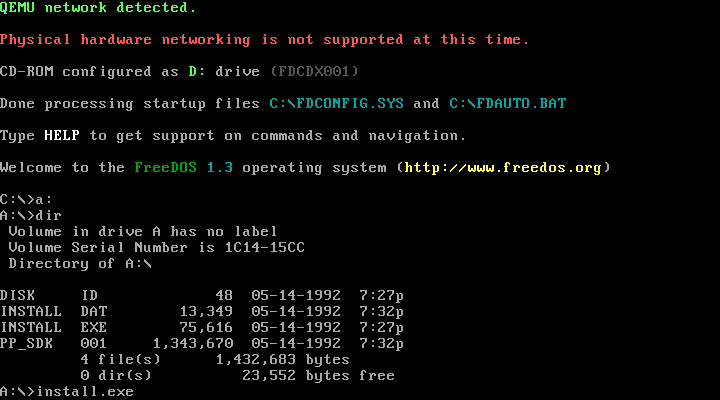
\includegraphics[width=0.9\linewidth]{fd-main-screen.png}
    \caption{FreeDOS: main screen}
    \label{fig:fd-main-screen}
\end{figure}

Then get through the installation wizard by confirming to use the C: drive for
installation and the installation subdirectory \ref{fig:penpoint-installation}.
The default choices are fine.  After installation from the first floppy is
finished the wizard will ask to insert the next disk until the contents of all
eight disks are installed.

\begin{figure}[H]
    \centering
    \begin{subfigure}[b]{0.45\linewidth}
        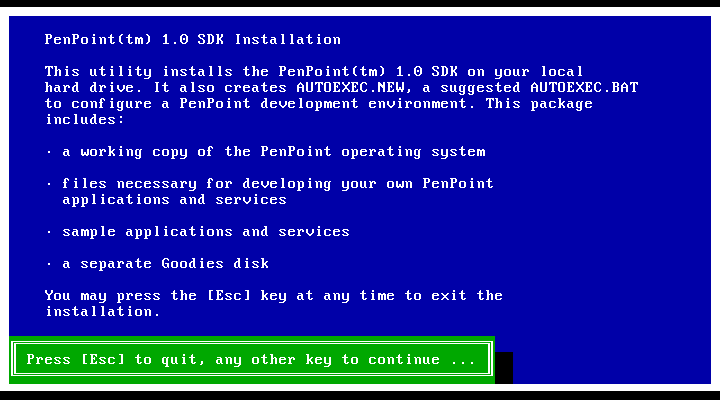
\includegraphics[width=\linewidth]{penpoint-installation-1.png}
        %\caption{PenPoint OS installation}
        %\label{fig:penpoint-installation-1}
    \end{subfigure}
    \hfill
    \begin{subfigure}[b]{0.45\linewidth}
        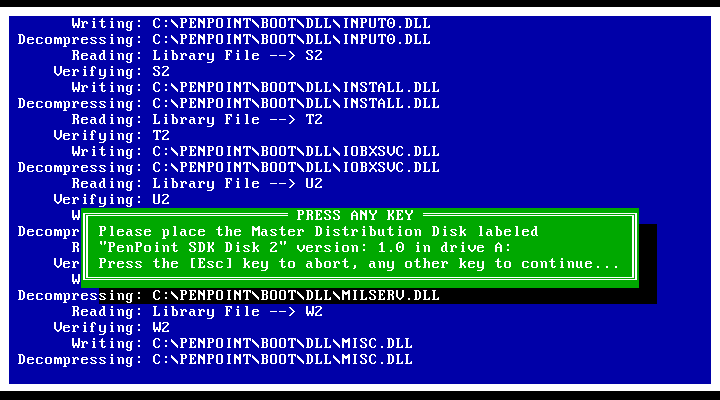
\includegraphics[width=\linewidth]{penpoint-installation-2.png}
        %\caption{PenPoint OS installation}
        %\label{fig:penpoint-instsallation-2}
    \end{subfigure}
    \caption{FreeDOS: PenPoint OS install wizard}
    \label{fig:penpoint-installation}
\end{figure}

Just before the installation wizard closes it informs that additional user
configuration will be required before running PenPoint OS will be possible. It
tries to create or modify an existing \emph{CONFIG.SYS} file with a directive
\emph{FILES=20} and creates a new file called AUTOEXEC.NEW that has to be
incorporated into an existing \emph{AUTOEXEC.BAT} file
\ref{fig:penpoint-installation-2}.

\begin{figure}[H]
    \centering
    \begin{subfigure}[b]{0.45\linewidth}
        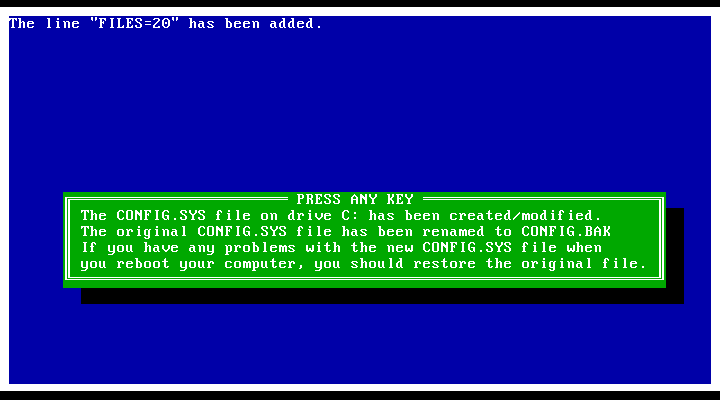
\includegraphics[width=\linewidth]{penpoint-installation-3.png}
        %\caption{PenPoint OS installation}
        %\label{fig:penpoint-installation-3}
    \end{subfigure}
    \hfill
    \begin{subfigure}[b]{0.45\linewidth}
        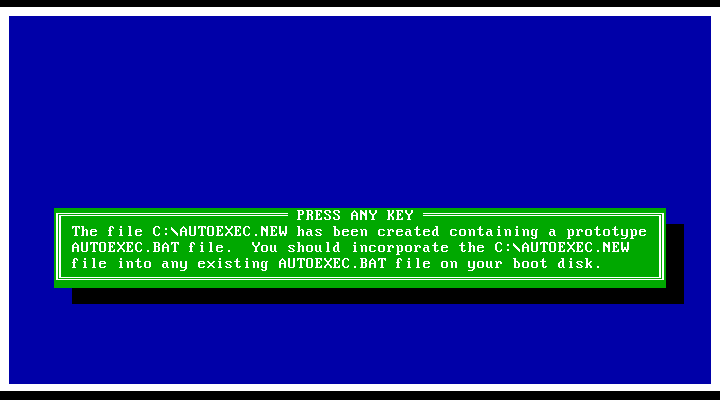
\includegraphics[width=\linewidth]{penpoint-installation-4.png}
        %\caption{PenPoint OS installation}
        %\label{fig:penpoint-instsallation-4}
    \end{subfigure}
    \caption{FreeDOS: PenPoint OS installation, config changes}
    \label{fig:penpoint-installation-2}
\end{figure}

FreeDOS actually by default uses \emph{FDCONF.SYS} and \emph{FDAUTO.BAT} files
instead. The config file is a special file that is run during startup and has
a special set of commands that can be run during boot. The \emph{FILES=20}
command sets the maximum number of file descriptors to 20. This is unnecessary
because default \emph{FDCONF.SYS} already uses a value of 40. The autoexec file
is a regular batch file that is automatically run after startup. The contents
of the \emph{AUTOEXEC.NEW} file are simply commands setting the environmental
variables used by PenPoint with paths from installation. These can be just
copied at the top of the \emph{FDAUTO.BAT} \ref{fig:fd-config}. It might be
useful to remember not to overwrite the \emph{PATH} variable but instead to
prepend the PenPoint value so that executables bundled with FreeDOS can still
be found.

\begin{figure}[H]
    \centering
    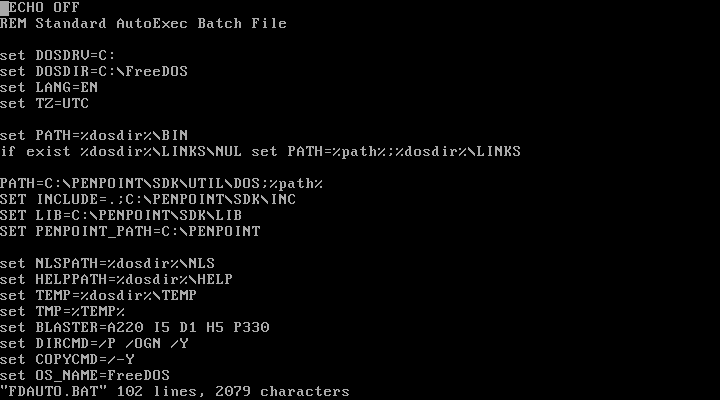
\includegraphics[width=0.9\linewidth]{fd-config.png}
    \caption{FreeDOS: FDAUTO.BAT config file}
    \label{fig:fd-config}
\end{figure}

Now we can try running PenPoint.

\subsection{Running PenPoint OS}

%Now that the installation is complete to run PenPoint a script
%\emph{\\
%\textbackslash{}PENPOINT\textbackslash{}SDK\textbackslash{}UTIL\\
%\textbackslash{}DOS\textbackslash{}GO.BAT\\
%} \\
Now that the installation is complete to run PenPoint a script

\Verb[fontshape=it]|\PENPOINT\SDK\UTIL\DOS\GO.BAT|

\noindent
should be used. Here however we encounter the first problem. PenPoint does not
start, instead it crashes with a JemmEx exception \ref{fig:jemmex}.

\begin{figure}[H]
    \centering
    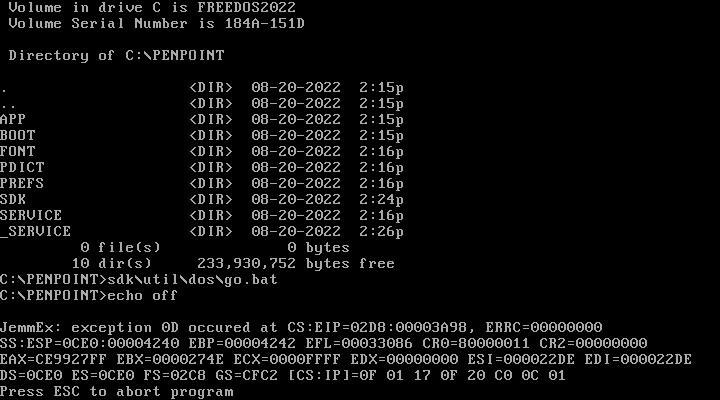
\includegraphics[width=0.9\linewidth]{jemmex.png}
    \caption{FreeDOS: JemmEx exception}
    \label{fig:jemmex}
\end{figure}

After trying a few things it turns out that this issue does not occur if FreeDOS
was booted in safe mode - one of the booting options defined in
\emph{FDCONF.SYS}. As it turns out JemmEx is in fact not loaded this way.
JemmEx is an Expanded Memory Manager. Expanded Memory was a workaround for 8088
and 8086 CPUs that allowed using the Upper Memory, that is between 640K and 1M
to address memory beyond 1M. Extended Memory on the other hand refers to memory
beyond the 1M on 286 and newer processors which could address this memory
normally. PenPoint OS does not support Expanded Memory and only works on Extended
Memory \cite{godevtools}.

Now after removing loading JemmEx from startup PenPoint OS starts. However there
is another problem. After some loading a broken pen and a number 1000 appears,
and the initialisation hangs \ref{fig:broken-pen}.

\begin{figure}[H]
    \centering
    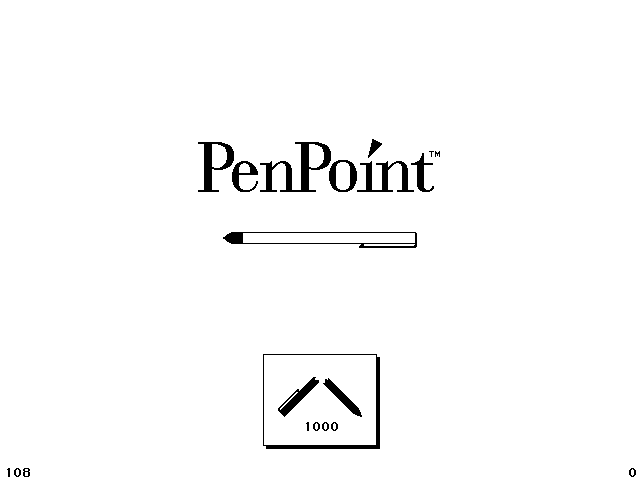
\includegraphics[width=0.9\linewidth]{broken-pen.png}
    \caption{PenPoint OS: broken pen error 1000}
    \label{fig:broken-pen}
\end{figure}

The error 1000 according to the ``Pen Point Development Tools'' book means that
no pointing device was enabled in the \emph{MIL.INI} file \cite{godevtools}.
After uncommenting the line that enables PS2 mouse support in \emph{MIL.INI}
\ref{fig:mil-ini}, PenPoint OS boots correctly \ref{fig:penpoint-mainscreen}.

\begin{figure}[H]
    \centering
    \begin{subfigure}[b]{0.45\linewidth}
        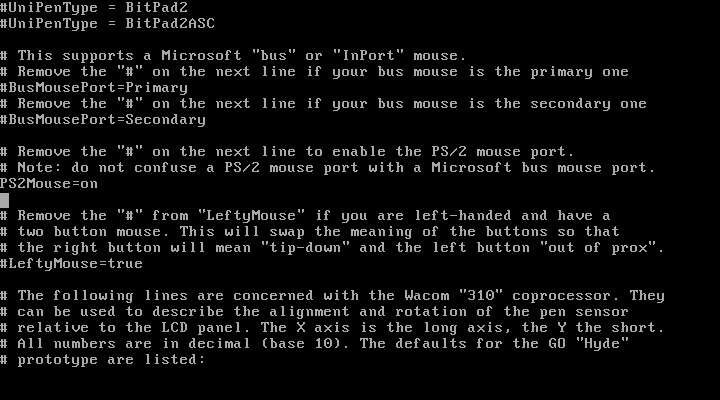
\includegraphics[width=\linewidth]{mil-ini.png}
        \caption{FreeDOS: MIL.INI}
        \label{fig:mil-ini}
    \end{subfigure}
    \hfill
    \begin{subfigure}[b]{0.45\linewidth}
        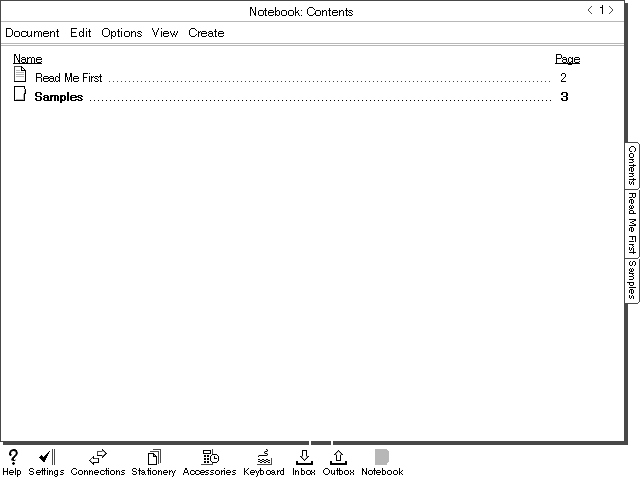
\includegraphics[width=\linewidth]{penpoint-mainscreen.png}
        \caption{PenPoint OS: main screen}
        \label{fig:penpoint-mainscreen}
    \end{subfigure}
    \caption{booted PenPoint OS}
\end{figure}

\subsection{Using a graphics tablet to point}

Now PenPoint is running and working correctly with a mouse.  Unfortunately just
because a mouse is working does not mean that other pointing devices will work
as well.  For example a mouse and a graphics tablet used with a finger work
without issue, but using a stylus is unwieldy.  Instead of moving with the pen
on the tablet, the pointer behaves more like a joystick - when the stylus is in
the middle of the tablet the pointer is stationary but when stylus is moved off
centre then the pointer moves in that direction, and the farther the stylus is
from the centre the faster it moves.  All of this happens because a mouse or
a finger movement on a tablet is a relative movement - the mouse moves by some
distance in a direction then the pointer should also move by that distance in
that direction, a stylus or a touchscreen, on the other hand, use absolute
movement - the stylus touches one corner of the tablet, the pointer should be
moved to the coroner of the screen.  The PS2 mouse emulation QEMU provides does
not have this functionality.

% TODO: \dots?
\begin{codeblock}
    \lstinputlisting[
        caption=ps2.c,
        language=C++,
        linerange={783-785,793-794,802-810,835-836},
    ]{ps2-old.c}
\end{codeblock}
%\begin{minipage}{\linewidth}
%    \begin{addmargin}[8mm]{0mm}
%        \begin{lstlisting}[
%            language=C++,
%            numbers=left,
%            firstnumber=1,
%            %    caption={\emph{Hello world} w HTML},
%            aboveskip=10pt,
%            %escapeinside=``,
%            breaklines=true,
%            ]
%static void ps2_mouse_event(DeviceState *dev, QemuConsole *src,
%                            InputEvent *evt)
%{
%    ...
%    PS2MouseState *s = (PS2MouseState *)dev;
%    InputMoveEvent *move;
%    ...
%
%    switch (evt->type) {
%    case INPUT_EVENT_KIND_REL:
%        move = evt->u.rel.data;
%        if (move->axis == INPUT_AXIS_X) {
%            s->mouse_dx += move->value;
%        } else if (move->axis == INPUT_AXIS_Y) {
%            s->mouse_dy -= move->value;
%        }
%        break;
%    ... 
%    }
%}
%        \end{lstlisting}
%    \end{addmargin}
%\end{minipage}

%QEMU also provides a graphics tablet emulation but it is a USB HID device that
%has to be initialised by the operating system. Simply adding a case handling an
%absolute movement to the PS2 mouse code, similar to the one in the source of
%the HID device, makes the mouse stop working altogether. It would probably have
%to keep a state where the pointer is and calculate the delta from there.
%
%
%\begin{minipage}{\linewidth}
%    \begin{addmargin}[8mm]{0mm}
%        \begin{lstlisting}[
%            language=C++,
%            numbers=left,
%            firstnumber=1,
%            %    caption={\emph{Hello world} w HTML},
%            aboveskip=10pt
%            ]
%    case INPUT_EVENT_KIND_ABS:
%        move = evt->u.abs.data;
%        if (move->axis == INPUT_AXIS_X) {
%            s->mouse_dx = move->value;
%        } else if (move->axis == INPUT_AXIS_Y) {
%            s->mouse_dy = move->value;
%        }
%        break;
%        \end{lstlisting}
%    \end{addmargin}
%\end{minipage}

%At this point in time it is impossible to get rid of this issue without a big
%time investment. 

%Fortunately u
Using both a mouse and a tablet works out of the box in a different
virtual machine program: VirtualBox. VirtualBox follows a more plug-and-play
philosophy at a cost of being generally slower than QEMU. It has much less
configuration options, is less optimised and does not provide support for such
functionality as using devices directly with passthrough. The developers of
VirtualBox have put an effort into it working without the need for much
configuration instead.% The incurred speed penalty from using VirtualBox and not
%QEMU to run PenPoint is not perceivable if it is there at all.




\clearpage % Rozdziały zaczynamy od nowej strony.

\section{Making tablet and stylus work in FreeDOS in QEMU}

% hid nie działa bo nie ma go kto zainicializować
% in the following section...

QEMU supports using tablet as a pointing device but it does not work in FreeDOS
because QEMU only provides a generic Human Interface Device (HID) driver.  The
USB-HID specification is a standard that allows for many different input and
output devices to communicate with the computer without any additional software.
For the QEMU HID device to work however it must be initialised by the operating
system.  DOS obviously came long before HID standard was created, and so it is
not supported by FreeDOS.

In this section I will describe the process of making the tablet behave as the
pointing device in the expected way inside FreeDOS on QEMU.

\subsection{Creating testing environment}

% używanie qemu bez trzymanki trudne

QEMU is extremely feature rich.  This is a great advantage, however it makes
using, tuning configuring it pretty cumbersome, especially since QEMU by itself
only provides console arguments as a way to specify settings.

\subsubsection{libvirt}

% co to libvirt, virsh, virt-manager

Libvirt is a collection of software whose goal is to provide simple, convenient
and unified way to manage virtualisation functionality such as virtual machines
and hypervisors, but also containers and network interfaces.  The pieces of
software that make up libvirt are a stable C API, a libvirtd daemon, and
a command line client virsh.

But virsh is not the only client.  The way libvirt operates anyone can use the
API to communicate with the daemon in their client.  Apart from virsh GOME
provides its own libvirt client - GOME Boxes - that matches the rest of their
environment, and there also exist an add-on to cockpit - the web-based server
administration tool.  I used virt-manager.

Here comes the problem however: although virt-manager proved to be great for
configuring amounts of memory, number of cores and adding peripherals, it does
not allow a way to change the path of the used QEMU executable, and overwriting
an executable provided and managed by the distribution's package manager is
something that could lead to serious issues.

\subsubsection{Using virsh}

% virsh dump cmd: zrzut
% virsh edit: zrzut
% sprawdzanie logów: zrzut

My first thought was to somehow find out the exact way that virt-manager
executes the QEMU binary, that is the command line parameters and maybe the
environment.  It turns out that every guest configuration is stored in xml
format in something called the domain.  It also turns out that the virsh command
line libvirt client has the ability to convert that xml to equivalent shell
invocation.

\begin{codeblock}
    \dots
    \lstinputlisting[
        caption={},
        language=bash,
        linerange={7-15},
        deletekeywords={local,wait},
    ]{virsh-domxml-to-native.sh}
    \dots
    \lstinputlisting[
        caption={},
        language=bash,
        linerange={29-36},
        deletekeywords={local,wait},
    ]{virsh-domxml-to-native.sh}
    \dots
    \lstinputlisting[
        caption={\lstinline|virsh domxml-to-native qemu-argv --domain PenPointOS|},
        language=bash,
        linerange={56-59},
        deletekeywords={local,wait},
    ]{virsh-domxml-to-native.sh}
\end{codeblock}

This however still did not work.  At the very least many of the paths for files
and directories that it used for example in the \lstinline{/var/lib/libvirt} are
dynamically created at runtime.  I tried copying them and adjusting the startup
script accordingly but it still would not cooperate.  This clearly was not the
right approach.

How about modifying the domain xml directly?  Fortunately virsh allows to do
this using the \emph{edit} command.

\begin{codeblock}
    \lstinputlisting[
        caption={},
        language=XML,
        linerange={1-16},
    ]{virsh-dumpxml.xml}

    \dots

    \lstinputlisting[
        caption={\lstinline|virsh edit PenPointOS|},
        language=XML,
        linerange={123-123},
    ]{virsh-dumpxml.xml}
\end{codeblock}

\noindent
Especially interesting is the line containing the \emph{emulator} tag.

\begin{codeblock}
    \lstinputlisting[
        caption={},
        language=XML,
        linerange={35-36},
    ]{virsh-dumpxml.xml}
    
    \dots

    \lstinputlisting[
        caption={\lstinline|virsh edit PenPointOS|},
        language=XML,
        linerange={122-123},
    ]{virsh-dumpxml.xml}
\end{codeblock}

\noindent
According to libvirt documentation \cite{libvirt} the \emph{emulator} element
specifies the fully qualified path to the emulator binary.

With this knowledge I was able to clone the QEMU virtual machine which had
FreeDOS with PenPoint SDK installed and change the binary that was used for
emulation to the one supplied by me.  This way I could have two virtual machines
that differed only in the QEMU binary they used which was useful as
a comparison.

\subsection{Building QEMU} %?

% info z aur
% configure
% make depends
% brak spice-protocol

When using QEMU in conjunction with other tools like libvirt it is important
that it is built with all the required functionality.  QEMU uses
a \emph{configure} script to determine local build environment characteristic.
%One way to increase the build speed is to configure the build environment to
%only compile the x86 system target.

\begin{codeblock}
    \begin{lstlisting}[
        caption={configure},
        language=bash,
        numbers=none,
        deletekeywords={enable},
    ]
        ../configure \
            --target-list=x86_64-softmmu \
            --sysconfdir=/etc --localstatedir=/var \
            --libexecdir=/usr/lib/qemu --smbd=/usr/bin/smbd \
            --enable-modules --enable-sdl --disable-werror
    \end{lstlisting}
\end{codeblock}

The \emph{virsh edit} command verifies correctness of the modified domain
configuration.  In my case it was able to detect that the newly built QEMU
binary was missing support for SPICE which virt-manager used for display and
input to that virtual machine, and I was able to fix it by installing a required
package.  A good way to find out how QEMU must be configured and its
dependencies is to inspect how a package for specified system is built.  On Arch
Linux one can easily read \emph{PKGBUILD} - a file describing the build process
- for \emph{qemu-git} package on Arch User Repository.

\subsection{Changes to QEMU source code}

% możliwość użycia tabletu w ppos, brak dokumentów itp.
% użycie ps2 do emulowania myszy
% opis ps2?
% centrum jest ui/input.c
%   w jaki sposób przekazuje info, skąd bierze, skąd wiadomo czy abs czy rel
% w moim przypadku dostaje info z ui/spice
% kod ps2

Although PenPoint supports multiple tablet devices, and even provides an option
to define a communication protocol for unsupported one \cite{godevtools}, I was
not able to find any information about graphical tablets from that time, much
less technical documentation that would be needed to create emulated version.

This however is not necessary.  Instead of creating a new device, a device that
is already present in QEMU and whose protocol is well supported - the PS/2 mouse
- can be used.  That is how Synaptic touchpad worked: when Synaptic drives that
supported absolute mode were not present the touchpad identified itself as
a mouse and used either PS/2, Serial or Apple Desktop Bus protocols
\cite{synapticsinterfacing}.

\subsubsection{PS/2 protocol}

Although the PS/2 protocol was introduced by IBM in 1987 the port was still
present on most of the desktop motherboards sold until just few years ago.
Over the years many extensions of the standard were created by the likes of
Logitech or Microsoft.

One such popular extensions is the Microsoft Intellimouse extensions which
allowed for use of scroll wheel or scroll wheel and five buttons instead of the
usual three \cite{ps2interface}.

Normally the PS/2 mouse sends information about its movement in a packet of
three bytes \ref{table:ps2packet3b}.

\begin{table}[H]
    \begin{tabular}{lllllllll}
        & bit 7 & bit 6 & bit 5 & bit 4 & bit 3 & bit 2 & bit 1 & bit 0 \\

        \cline{2-9} 

        \multicolumn{1}{l|}{byte 1}        & \multicolumn{1}{l|}{Y overflow}   &
        \multicolumn{1}{l|}{X overflow}    & \multicolumn{1}{l|}{Y sign}       &
        \multicolumn{1}{l|}{X sign}        & \multicolumn{1}{l|}{always 1}     &
        \multicolumn{1}{l|}{M btn} & \multicolumn{1}{l|}{R btn} &
        \multicolumn{1}{l|}{L btn} \\

        \cline{2-9} 

        \multicolumn{1}{l|}{byte 2} & \multicolumn{8}{c|}{X movement} \\

        \cline{2-9} 

        \multicolumn{1}{l|}{byte 3} & \multicolumn{8}{c|}{Y movement} \\

        \cline{2-9} 
    \end{tabular}
    \caption{PS/2 mouse packet \cite{ps2interface}}
    \label{table:ps2packet3b}
\end{table}

\noindent
In order to enable the Intellimouse extensions the mouse sends a sequence of
three `Set sample rate' commands with predefined magic values.  A driver
compatible with that extension replies by issuing a `Get device ID' command to
which the mouse will respond with ID of 0x03.  Now both devices switch to using
four byte packets \ref{table:imps2scroll} \ref{table:imps25buttons}.

\begin{table}[H]
    \begin{tabular}{lllllllll}
        & bit 7 & bit 6 & bit 5 & bit 4 & bit 3 & bit 2 & bit 1 & bit 0 \\

        \cline{2-9} 

        \multicolumn{1}{l|}{byte 1}        & \multicolumn{1}{l|}{Y overflow}   &
        \multicolumn{1}{l|}{X overflow}    & \multicolumn{1}{l|}{Y sign}       &
        \multicolumn{1}{l|}{X sign}        & \multicolumn{1}{l|}{always 1}     &
        \multicolumn{1}{l|}{M btn} & \multicolumn{1}{l|}{R btn} &
        \multicolumn{1}{l|}{L btn} \\

        \cline{2-9} 

        \multicolumn{1}{l|}{byte 2} & \multicolumn{8}{c|}{X movement} \\

        \cline{2-9} 

        \multicolumn{1}{l|}{byte 3} & \multicolumn{8}{c|}{Y movement} \\

        \cline{2-9} 

        \multicolumn{1}{l|}{byte 4} & \multicolumn{8}{c|}{Z movement} \\

        \cline{2-9} 
    \end{tabular}
    \caption{Intellimouse PS/2 mouse with scroll wheel packet \cite{ps2interface}}
    \label{table:imps2scroll}
\end{table}

\noindent
and

\begin{table}[H]
    \begin{tabular}{lllllllll}
        & bit 7 & bit 6 & bit 5 & bit 4 & bit 3 & bit 2 & bit 1 & bit 0 \\

        \cline{2-9} 

        \multicolumn{1}{l|}{byte 1}     & \multicolumn{1}{l|}{Y overflow}   &
        \multicolumn{1}{l|}{X overflow} & \multicolumn{1}{l|}{Y sign}       &
        \multicolumn{1}{l|}{X sign}     & \multicolumn{1}{l|}{always 1}     &
        \multicolumn{1}{l|}{M btn}      & \multicolumn{1}{l|}{R btn}        &
        \multicolumn{1}{l|}{L btn} \\

        \cline{2-9} 

        \multicolumn{1}{l|}{byte 2} & \multicolumn{8}{c|}{X movement} \\

        \cline{2-9} 

        \multicolumn{1}{l|}{byte 3} & \multicolumn{8}{c|}{Y movement} \\

        \cline{2-9} 

        \multicolumn{1}{l|}{byte 4}     & \multicolumn{2}{c|}{always 0} &
        \multicolumn{1}{l|}{5th btn}    & \multicolumn{1}{l|}{4th btn}  &
        \multicolumn{4}{c|}{Z movement} \\

        \cline{2-9} 
    \end{tabular}
    \caption{Intellimouse PS/2 mouse with scroll wheel + 5 buttons packet \cite{ps2interface}}
    \label{table:imps25buttons}
\end{table}

\noindent
The QEMU PS/2 mouse device supports both of these extensions.

%There does not seem to be any current publication of the standard
%\cite{ps2interface}.

\subsubsection{SPICE initialization}

SPICE project is a software solution that aims to provide remote-display to
virtual environments, on the same computer or anywhere on the internet.  It is
comprised of the SPICE protocol, server, and several client implementations are
available.  The \emph{virt-manager} program uses either SPICE or VNC to provide
display and pointer input, and QEMU is compatible also with other sources.  The
description of SPICE is ilustratory. % TODO

QEMU defines a SPICE module.

\begin{codeblock}
    \lstinputlisting[
        caption=spice-core.c,
        language=C,
        linerange={968-985},
    ]{spice-core.c}
\end{codeblock}

Inside the \emph{qemu\_spice\_init} function \emph{qemu\_spice\_input\_init}
function is called.

\begin{codeblock}
    \lstinputlisting[
        caption={},
        language=C,
        linerange={640-641},
    ]{spice-core.c}
    \dots
    \lstinputlisting[
        caption={},
        language=C,
        linerange={827-827},
    ]{spice-core.c}
    \dots
    \lstinputlisting[
        caption=spice-core.c,
        language=C,
        linerange={852-852},
    ]{spice-core.c}
\end{codeblock}

The \emph{qemu\_spice\_input\_init} function adds the keyboard and mouse
interfaces, and adds and calls a mouse mode notifier.

\begin{codeblock}
    \lstinputlisting[
        caption=spice-input.c,
        language=C,
        linerange={243-262},
    ]{spice-input.c}
\end{codeblock}

The \emph{mouse\_mode\_notifier} adds a SPICE tablet interface if there is an
input handler with absolute mode available.

\begin{codeblock}
    \lstinputlisting[
        caption=spice-input.c,
        language=C,
        linerange={226-241},
    ]{spice-input.c}
\end{codeblock}

The function \emph{qemu\_input\_is\_absolute} simply checks if any of the
registered input handlers has the \emph{INPUT\_EVENT\_MASK\_ABS} flag set.

\begin{codeblock}
    \lstinputlisting[
        caption=input.c,
        language=C,
        linerange={493-500},
    ]{input.c}
\end{codeblock}

\subsubsection{PS/2 input device initialization}

The QEMU PS/2 mouse is registered using the standard QEMU interface for adding
devices.

% static const TypeInfo ps2_mouse_info
% ps2_info 
% ps2_register_types
% type_init
\begin{codeblock}
    \lstinputlisting[
        caption={ps2.c},
        language=C,
        linerange={1309-1315,1331-1339,1341-1346,1348-1348},
    ]{ps2-new.c}
\end{codeblock}

The \emph{ps2\_info} is used as a base type for both PS/2 mouse and keyboard.
Inside the PS/2 mouse class initialization function a realization function is
set to register the PS/2 mouse device as an input handler.

% ps2_mouse_realize
% ps2_mouse_class_init
\begin{codeblock}
    \lstinputlisting[
        caption={ps2.c},
        language=C,
        linerange={1276-1279,1298-1307},
    ]{ps2-new.c}
\end{codeblock}

\noindent
The reset function sets all of the device state to the initial values, and the
VM state description structure is used to provide a mechanism to save and
restore the state of all devices.

The \emph{qemu\_input\_handler\_register} function is called with a struct that
describes the capabilities of the mouse and callbacks for events and syncing.
Here the \emph{INPUT\_EVENT\_MASK\_ABS} is added to indicate that the PS/2 mouse
can work in absolute mode.  Setting this flag will make it so that the SPICE
tablet interface is added, and absolute mode events will be handled by the PS/2
mouse device.

% ps2_mouse_handler
\begin{codeblock}
    \lstinputlisting[
        caption=ps2.c,
        language=C,
        linerange={1269-1279},
    ]{ps2-new.c}
\end{codeblock}

\subsubsection{How input in QEMU is processed}

When pointer position changes SPICE uses either mouse or tablet interfaces that
were initialised in the \emph{qemu\_spice\_input\_init} function.  If absolute
input handler is available the tablet interface is used for absolute pointer
% TODO czy tylko?
position changes.

\begin{codeblock}
    \lstinputlisting[
        caption=spice-input.c,
        language=C,
        linerange={215-224},
    ]{spice-input.c}
\end{codeblock}

SPICE calls the \emph{tablet\_position} function using the \emph{position}
member of the tablet interface.

\begin{codeblock}
    \lstinputlisting[
        caption=spice-input.c,
        language=C,
        linerange={184-194},
    ]{spice-input.c}
\end{codeblock}

\noindent
The \emph{tablet\_position} queues the absolute input for both axes and issues
the event sync.

The \emph{qemu\_input\_queue\_abs} scales the input value and sends the event.
The \emph{qemu\_input\_send\_event} function performs some checks and calls the
\emph{replay\_input\_event}, which adds the event to replay if in replay mode,
and otherwise it calls the \emph{qemu\_input\_send\_event\_impl}.  Finally this
function finds an appropriate input handler and calls its event callback.

\begin{codeblock}
    \lstinputlisting[
        caption={},
        language=C,
        linerange={529-543},
    ]{input.c}
    \lstinputlisting[
        caption={},
        language=C,
        linerange={353-354,378-379},
    ]{input.c}
    \lstinputlisting[
        caption=input.c,
        language=C,
        linerange={333-334,345-351},
    ]{input.c}
\end{codeblock}

\noindent
The event sync functionality is implemented similarly ending in calling the
input handler callback for syncing.

\subsubsection{Emulation of absolute input using PS/2 mouse device}

Because the PS/2 mouse protocol uses relative pointer mode - that is it
transfers by how much the mouse moved from the last position - and a tablet
provides values in absolute mode - that is it reports the current absolute
stylus position - the absolute mode values must be converted to relative terms
somehow.  To do so the mouse device structure should hold the last known
absolute position.  Whenever an event occurs the last known absolute position
would be updated, and when handling an event with absolute movement the position
difference could be calculated and communicated using the standard PS/2
protocol.

The fields \emph{absolute\_x} and \emph{absolute\_y} are added to the
\emph{PS2MouseState} structure.

%\begin{codeblock}
%    \begin{lstlisting}[
%        caption=ps2.h,
%        language=C,
%        escapechar=!,
%    ]
%struct PS2MouseState {
%    PS2State parent_obj;
%
%    uint8_t mouse_status;
%    uint8_t mouse_resolution;
%    uint8_t mouse_sample_rate;
%    uint8_t mouse_wrap;
%    uint8_t mouse_type; /* 0 = PS2, 3 = IMPS/2, 4 = IMEX */
%    uint8_t mouse_detect_state;
%    int mouse_dx; /* current values, needed for 'poll' mode */
%    int mouse_dy;
%    int mouse_dz;
%    int mouse_dw;
%    !\colorbox{green}{{int absolute\_x;}}!
%    !\colorbox{green}{{int absolute\_y;}}!
%    uint8_t mouse_buttons;
%};
%    \end{lstlisting}
%\end{codeblock}

\begin{codeblock}
    \lstinputlisting[
        caption=ps2.h,
        language=C,
        linerange={81-97},
    ]{ps2-new.h}
\end{codeblock}

They are also added to the reset function, and the \emph{VMStateDescription}
struct.

\begin{codeblock}
    \lstinputlisting[
        caption=ps2.c,
        language=C,
        linerange={1091-1112,1234-1256}
    ]{ps2-new.c}
\end{codeblock}

The \emph{INPUT\_EVENT\_MASK\_ABS} flag is also set for the PS/2 mouse input
handler.  This makes it so that QEMU recognizes that it can handle absolute
input, and that SPICE registers the tablet interface.  Then events with absolute
movement are sent to the PS/2 mouse input handler \emph{event} function.

\begin{codeblock}
    \lstinputlisting[
        caption=ps2.c,
        language=C,
        linerange={1269-1274},
    ]{ps2-new.c}
\end{codeblock}

Finally the code that updates the current known absolute position, and
calculates the absolute movement deltas is added to the \emph{ps2\_mouse\_event}
function.

\begin{codeblock}
    \lstinputlisting[
        caption=ps2.c,
        language=C,
        linerange={783-785,802-848,873-874},
    ]{ps2-new.c}
\end{codeblock}


\subsection{Tying it all together}

% website about how to install everything

Following the process of installation and using the modified QEMU version allows
to use PenPoint OS SDK version with a graphics tablet and stylus.  A detailed
step-by-step guide and all of the necessary files are available on my website at
\url{khnsky.github.io/qemu-penpointos/}
